\documentclass[letterpaper,11pt]{article}
\oddsidemargin -1.0cm \textwidth 17.5cm

\usepackage[utf8]{inputenc}
\usepackage[activeacute,spanish, es-lcroman]{babel}
\decimalpoint
\usepackage{amsfonts,setspace}
\usepackage{amsmath}
\usepackage{amssymb, amsmath, amsthm}
\usepackage{comment}
\usepackage{float}
\usepackage{amssymb}
\usepackage{dsfont}
\usepackage{anysize}
\usepackage{multicol}
\usepackage{enumerate}
\usepackage{graphicx}
\usepackage[left=1.5cm,top=1.5cm,right=1.5cm, bottom=1.7cm]{geometry}
\setlength\headheight{1.5em} 
\usepackage{fancyhdr}
\usepackage{multicol}
\usepackage{hyperref}
\usepackage{wrapfig}
\usepackage{subcaption}
\usepackage{siunitx}
\usepackage{cancel}
\pagestyle{fancy}
\fancyhf{}
\renewcommand{\labelenumi}{\normalsize\bfseries P\arabic{enumi}.}
\renewcommand{\labelenumii}{\normalsize\bfseries (\alph{enumii})}
\renewcommand{\labelenumiii}{\normalsize\bfseries \roman{enumiii})}

\begin{document}

\fancyhead[L]{\itshape{Facultad de Ciencias F\'isicas y Matem\'aticas}}
\fancyhead[R]{\itshape{Universidad de Chile}}

\begin{minipage}{11.5cm}
    \begin{flushleft}
        \hspace*{-0.6cm}\textbf{FI1100 Introducción a la Física Moderna}
    \end{flushleft}
\end{minipage}

\begin{picture}(2,3)
    \put(366, -10){
\includegraphics[scale=0.9]{Imágenes/logo/dfi-fcfm.pdf}}
\end{picture}

\begin{center}
	\LARGE\textbf{Problemitas de interferencia y difracción}
\end{center}

\vspace{-1cm}

\section*{\underline{Interferencia}}
\begin{enumerate}\setlength{\itemsep}{0.4cm}

\rfoot[]{pág. \thepage}

\item Dos antenas de radio separadas 300 m transmiten simultáneamente señales idénticas a la misma longitud de onda. El radio en un automóvil que se desplaza al norte recibe estas señales. \textbf{a)} Si el vehículo se encuentra en la posición del segundo máximo, ¿cuál es la longitud de onda de las señales? \textbf{b)} ¿Cuánto más lejos debe viajar el auto para encontrar el siguiente mínimo en recepción? (Nota: No utilice la aproximación de ángulo pequeño en este problema.)

\begin{figure}[H]
    \centering
    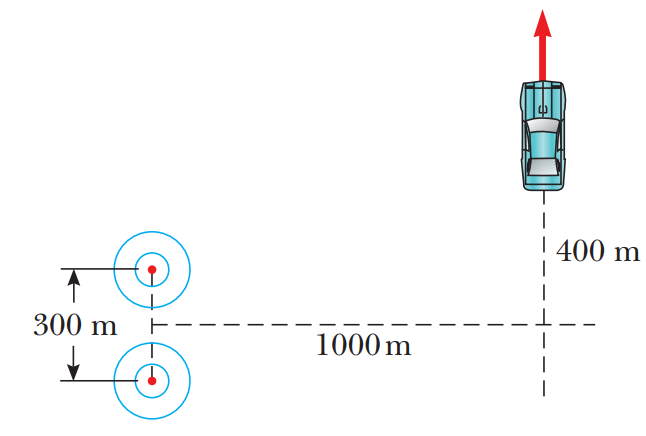
\includegraphics[width=0.4\linewidth]{Imágenes/clases/auto.png}
\end{figure}

\item Por un sistema de doble ranura que tiene una separación entre
ranuras $d = \SI{0.400}{\mm}$ pasa luz de $\SI{442}{\nm}$ de longitud de onda. Determine a qué distancia debe ponerse una pantalla para que
aparezca una franja oscura directamente opuesta a ambas ranuras, con sólo un franja brillante entre ellas.

\item Una cuña de aire se forma entre dos placas de vidrio separadas
por un alambre muy fino. Cuando la cuña es iluminada desde arriba por una luz de $\SI{600}{\nm}$ y se observa desde arriba, aparecen 30 franjas oscuras. Calcule el radio del alambre

\begin{figure}[H]
    \centering
    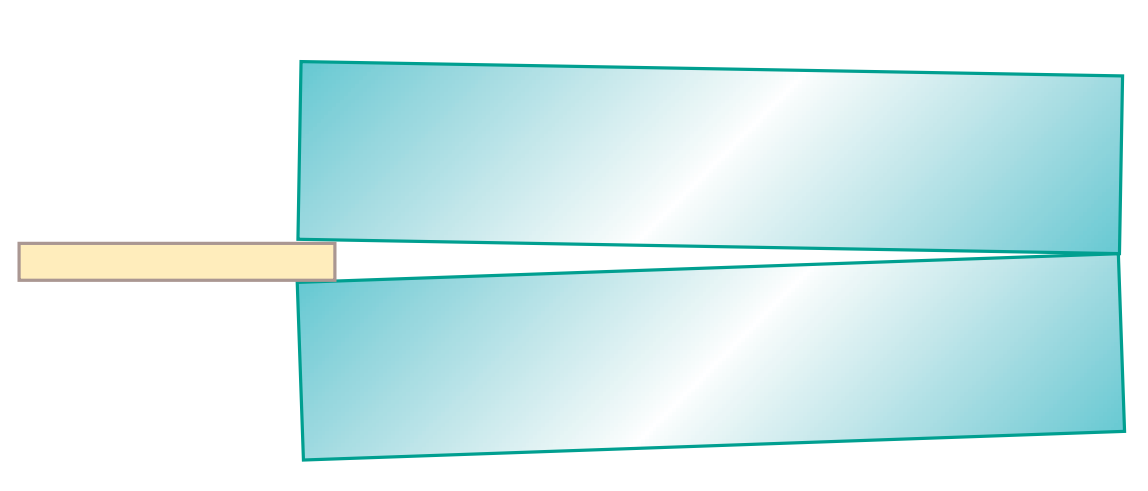
\includegraphics[width=0.3\linewidth]{Imágenes/clases/placas2.png}
\end{figure}

\item \textbf{[P2-C3 2020-2]} Se realiza un experimento de doble rendija usando un láser de He-Ne ($\lambda = \SI{633}{\nm}$). Luego, se coloca un placa muy delgada de vidrio ($n = 1.5$) sobre una de las ranuras. Se observa que el punto central en la pantalla está ahora ocupado por la que había sido la franja oscura correspondiente a $m = 10$. ¿Cuán grueso es el vidrio?
Considere que la pantalla está ubicada muy lejos, de manera que vale la aproximación paraxial (todos los ángulos son muy pequeños).

\item Una luz con una longitud de onda de $\SI{580}{\nm}$ incide sobre una rendija con un ancho de $\SI{0.300}{\mm}$. La pantalla de observación está a $\SI{2.00}{m}$ de la rendija. Determine las posiciones de las primeras franjas oscuras, así como el ancho de la franja central brillante.

\end{enumerate}
\end{document}